
\section{Mục tiêu đặt ra}

Mục tiêu của bài toán là xây dựng một \textbf{dashboard trực quan} nhằm khai thác và trình bày các \textbf{dữ liệu nội bộ} hiện có của hệ thống. Các trực quan tập trung vào những khía cạnh quan trọng của dữ liệu, bao gồm: \textit{số lượng và tình trạng xe}, \textit{thông tin theo từng hãng xe}, \textit{người bán/đại lý}, cũng như \textit{các bình luận và đánh giá của người dùng}.  

Dashboard được thiết kế nhằm hỗ trợ việc \textbf{theo dõi tổng quan}, \textbf{phân tích chi tiết} và \textbf{ra quyết định} dựa trên dữ liệu.

\section{Import, làm sạch và trực quan hóa dữ liệu}

\subsection{Import và làm sạch dữ liệu}

Sau bước tiền xử lý, dữ liệu được lưu dưới dạng các tệp \texttt{CSV} và được \textbf{kết nối trực tiếp vào Power BI}. Quá trình làm sạch và chuẩn hóa dữ liệu được thực hiện thông qua \textbf{Power Query}, với các bước chính như sau:
\begin{itemize}
    \item Chỉ giữ lại các cột cần thiết cho mục đích trực quan hóa trong từng tệp CSV (ví dụ: \texttt{vehicle\_id}, \texttt{condition}, \texttt{price}, \texttt{model\_name}, \ldots).
    \item Phân tách và tạo thêm các cột mới mang tính thông tin cao từ các cột ban đầu (ví dụ: \texttt{vehicle\_brand}, \texttt{year\_released}, \ldots), đồng thời loại bỏ các giá trị lỗi hoặc không hợp lệ.
    \item Xây dựng một bảng tổng hợp \texttt{Merged\_table} nhằm liên kết các bảng con, qua đó cho phép \textbf{tương tác (interaction)} giữa các biểu đồ trong dashboard.
\end{itemize}

\subsection{Trực quan hóa và phân tích cơ bản}

Sau khi hoàn tất quá trình import và làm sạch dữ liệu, các biểu đồ trực quan được xây dựng và tổ chức thành ba sheet chính, bao gồm: \textbf{OVERVIEW}, \textbf{NEW VEHICLES} và \textbf{USED VEHICLES}.

\subsubsection{Sheet OVERVIEW}

\begin{figure}[!htbp]
    \centering
    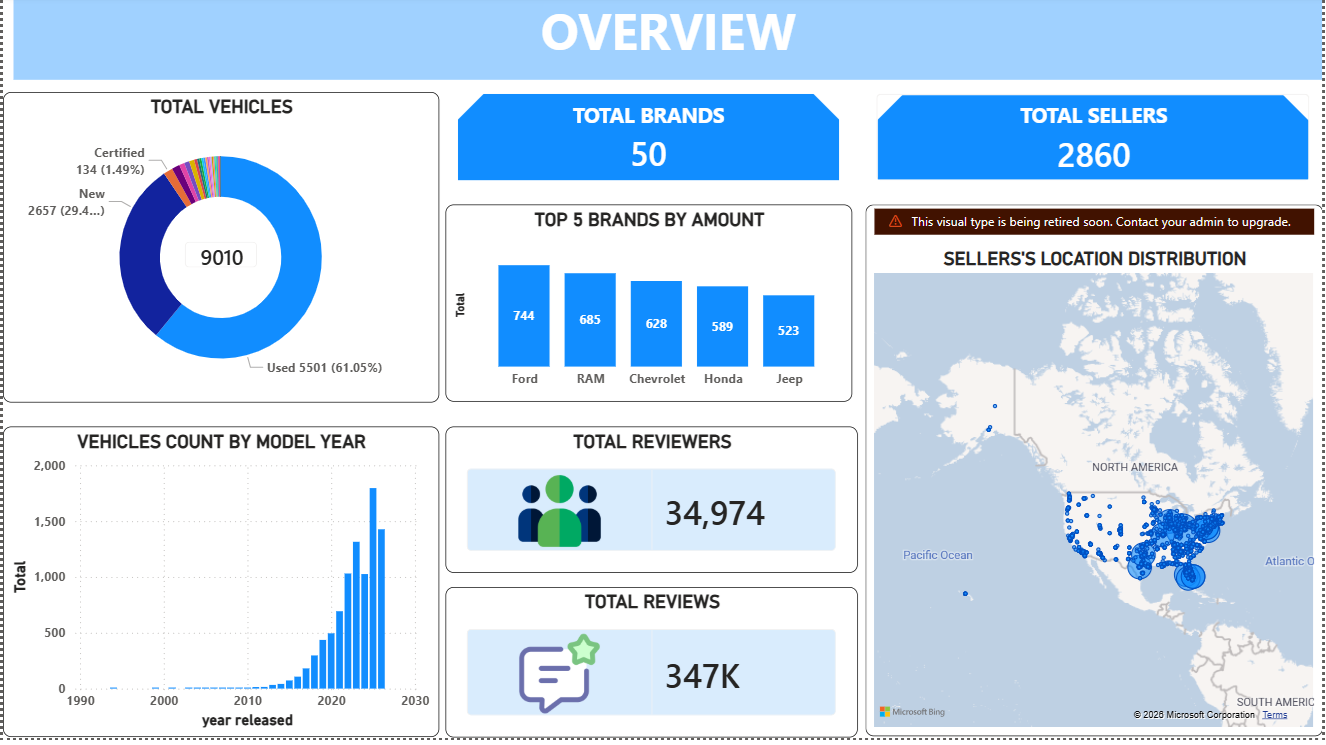
\includegraphics[width=0.9\textwidth]{images/OVERVIEW.png}
    \caption{Sheet OVERVIEW}
    \label{fig:overview}
\end{figure}


\noindent Phân tích tổng quan cho thấy:
\begin{itemize}
    \item Hệ thống ghi nhận tổng cộng \textbf{9,010 xe}, trong đó nhóm xe cũ chiếm hơn \textbf{60\%}, nhóm xe mới chiếm gần \textbf{30\%}, phần còn lại thuộc các nhóm khác.
    \item Dữ liệu bao gồm \textbf{50 hãng xe} khác nhau, được phân phối qua \textbf{2,860 đại lý/người bán}. Phần lớn các đại lý tập trung ở \textbf{khu vực phía Đông Hoa Kỳ}, trong khi khu vực phía Tây chỉ ghi nhận số lượng hạn chế.
    \item Năm hãng xe phổ biến nhất lần lượt là \textbf{Ford (744 xe)}, \textbf{Ram (685 xe)}, \textbf{Chevrolet (628 xe)}, \textbf{Honda (589 xe)} và \textbf{Jeep (523 xe)}.
    \item Phần lớn các mẫu xe có năm ra mắt từ \textbf{2020 trở về sau}, trong đó các mẫu thuộc năm \textbf{2025} chiếm số lượng lớn nhất.
    \item Tổng số lượng người đánh giá là \textbf{34,974}, đóng góp khoảng \textbf{347,000 lượt bình luận}.
\end{itemize}

\subsubsection{Sheet NEW VEHICLES}

\begin{figure}[!htbp]
    \centering
    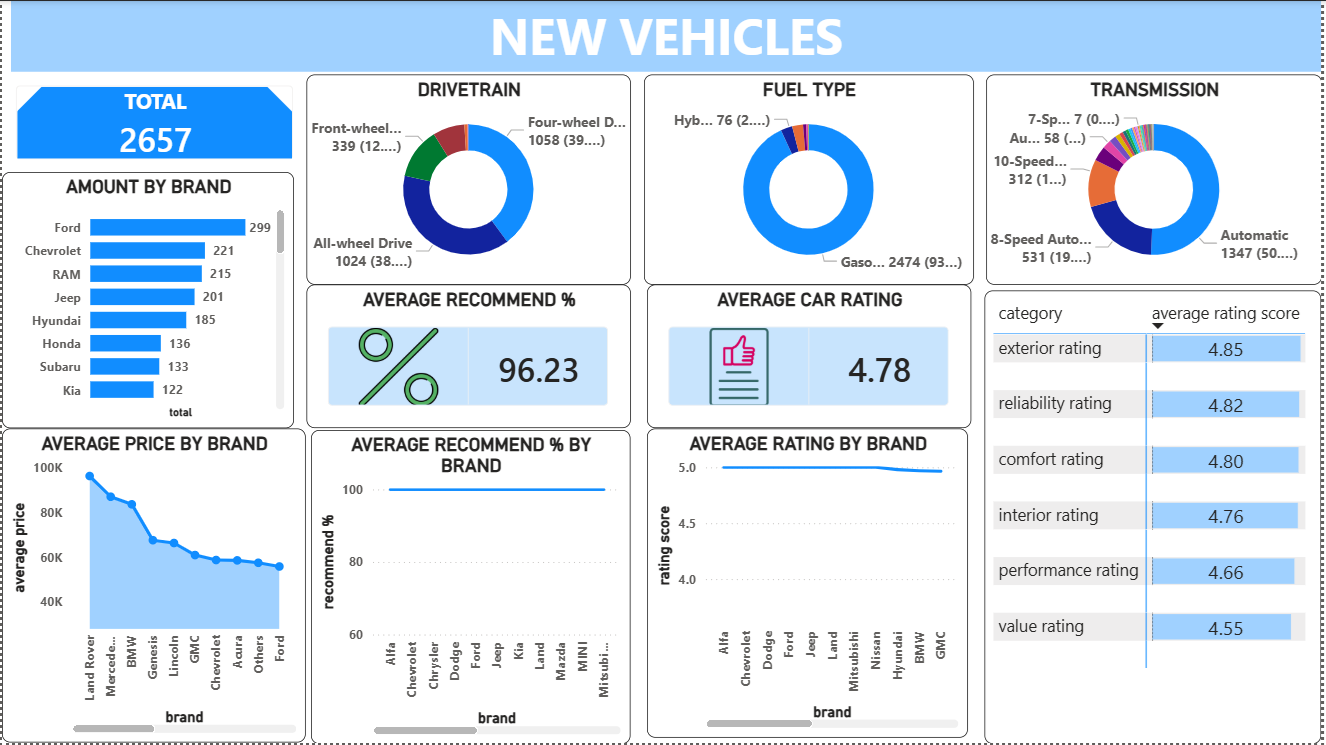
\includegraphics[width=0.9\textwidth]{images/NEW VEHICLES.png}
    \caption{Sheet NEW VEHICLES}
    \label{fig:new}
\end{figure}


\noindent Đối với nhóm xe mới, các đặc điểm nổi bật bao gồm:
\begin{itemize}
    \item Tổng số \textbf{2,657 xe mới}, trong đó hãng Ford chiếm tỷ trọng lớn nhất với \textbf{299 xe}, theo sau là Chevrolet và Ram.
    \item Hai hệ thống dẫn động phổ biến nhất là \textit{All-Wheel Drive} và \textit{Four-Wheel Drive}, mỗi loại chiếm gần \textbf{40\%} tổng số xe mới.
    \item Nhiên liệu được sử dụng chủ yếu là \textbf{xăng (Gasoline)}, chiếm hơn \textbf{90\%}.
    \item Hộp số phổ biến nhất là \textbf{Automatic}, theo sau là các biến thể \textbf{8-speed automatic} và \textbf{10-speed automatic}. Điều này cho thấy các nhà sản xuất ưu tiên mạnh mẽ hộp số tự động ở các dòng xe mới.
    \item Giá bán trung bình cao nhất thuộc về các hãng xe sang như \textbf{Land Rover} (gần 100,000 USD), \textbf{Mercedes-Benz} và \textbf{BMW} (trên 80,000 USD). Ngược lại, các hãng xe phổ thông như \textbf{Honda}, \textbf{Ford} và \textbf{Hyundai} có mức giá trung bình thấp hơn đáng kể (dưới 60,000 USD).
    \item Điểm đánh giá trung bình của xe mới đạt \textbf{4.78/5}. Một số hãng như \textbf{Alfa}, \textbf{Chevrolet} và \textbf{Dodge} đạt điểm tuyệt đối \textbf{5/5}, trong khi \textbf{Buick}, \textbf{Lincoln} và \textbf{Volkswagen} có mức đánh giá thấp hơn (dưới 4/5).
    \item Tỷ lệ đề xuất mua trung bình đạt \textbf{96.23\%}, phản ánh mức độ hài lòng rất cao. Các hãng như \textbf{Alfa}, \textbf{Chevrolet} và \textbf{Chrysler} đạt tỷ lệ đề xuất \textbf{100\%}, trong khi \textbf{Buick} và \textbf{Lincoln} là hai hãng duy nhất dưới 70\%.
    \item Ở mức đánh giá theo từng tiêu chí, \textbf{ngoại thất (exterior)}, \textbf{độ tin cậy (reliability)} và \textbf{độ thoải mái (comfort)} là ba tiêu chí có điểm số cao nhất (trên 4.80).
\end{itemize}

\subsubsection{Sheet USED VEHICLES}

\begin{figure}[!htbp]
    \centering
    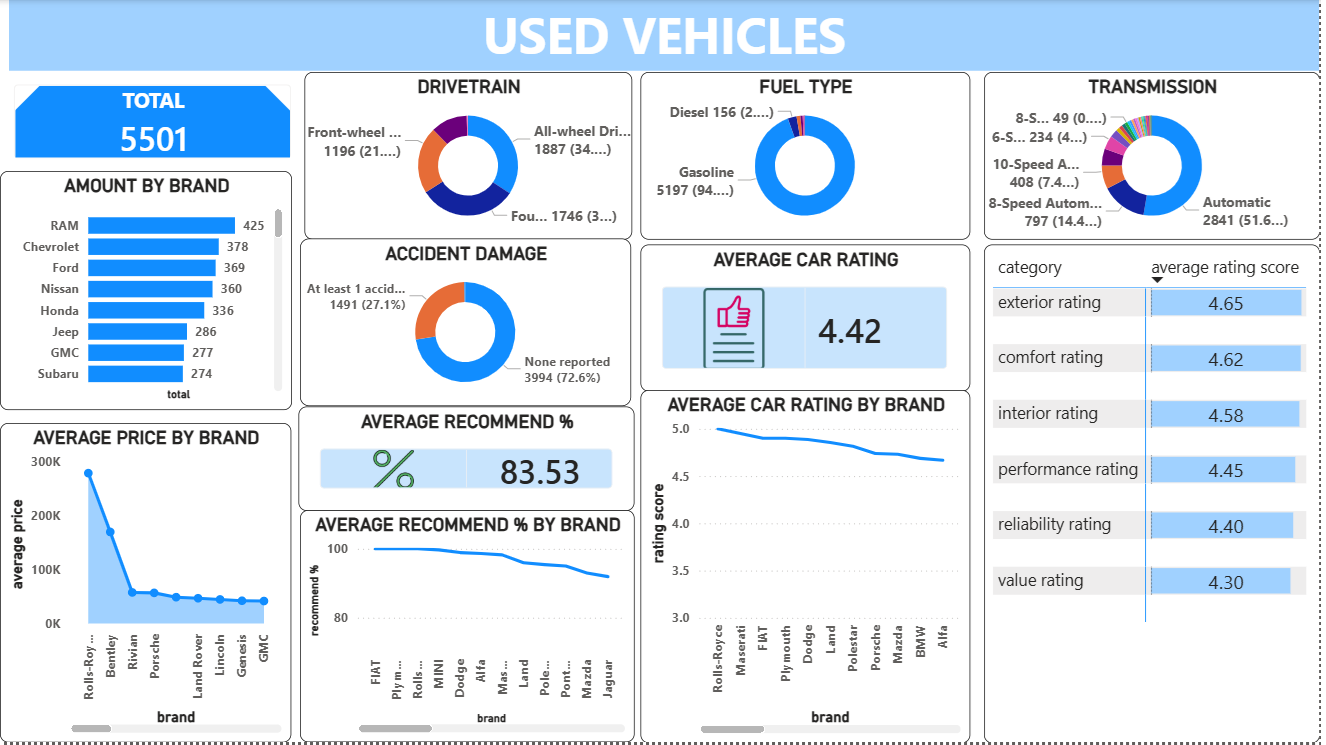
\includegraphics[width=0.9\textwidth]{images/USED VEHICLES.png}
    \caption{Sheet USED VEHICLES}
    \label{fig:used}
\end{figure}


\noindent Phân tích nhóm xe cũ cho thấy:
\begin{itemize}
    \item Tổng số \textbf{5,501 xe cũ}, trong đó các hãng Ram, Chevrolet và Ford chiếm tỷ trọng lớn nhất.
    \item Ba hệ thống dẫn động phổ biến nhất là \textit{All-Wheel Drive}, \textit{Four-Wheel Drive} và \textit{Front-Wheel Drive}, mỗi loại đều chiếm hơn \textbf{20\%}.
    \item Nhiên liệu được sử dụng chủ yếu vẫn là \textbf{Gasoline}.
    \item Hộp số phổ biến nhất là \textbf{Automatic}, tiếp theo là \textbf{8-speed automatic} và \textbf{10-speed automatic}.
    \item Tỷ lệ xe từng ghi nhận thiệt hại do tai nạn vào khoảng \textbf{30\%}.
    \item Giá bán trung bình cao nhất thuộc về các hãng xe sang như \textbf{Rolls-Royce} (gần 300,000 USD), \textbf{Bentley} và \textbf{Rivian}, trong khi phần lớn các hãng còn lại có giá trung bình dưới 60,000 USD.
    \item Tỷ lệ đề xuất mua trung bình đạt \textbf{83.53\%}, thấp hơn rõ rệt so với nhóm xe mới. Các hãng như \textbf{FIAT}, \textbf{Plymouth} và \textbf{Rolls-Royce} đạt mức đề xuất gần 100\%, trong khi một số hãng phổ thông như \textbf{Tesla}, \textbf{Volkswagen} và \textbf{Nissan} có tỷ lệ dưới 80\%.
    \item Điểm đánh giá trung bình của xe cũ đạt \textbf{4.42/5}, trong đó các hãng xe sang như \textbf{Rolls-Royce}, \textbf{Maserati} và \textbf{FIAT} có điểm số nổi bật.
    \item Ở mức đánh giá theo từng tiêu chí, \textbf{ngoại thất} và \textbf{độ thoải mái} tiếp tục là hai tiêu chí có điểm số cao nhất.
\end{itemize}
